\paragraph{}

Podczas prac nad programem zmianom uległy podstawowe założenia silnika graficznego, co miało znaczący wpływ na architekturę programu. Niektóre moduły wypadły zupełnie, niektóre zostały zmienione, a jeszcze inne dodane. Poniżej znajduje się nowy diagram modułów, oraz opis tych które są nowe, bądź uległy zmianie.

\begin{figure}[ht!]
\centering
	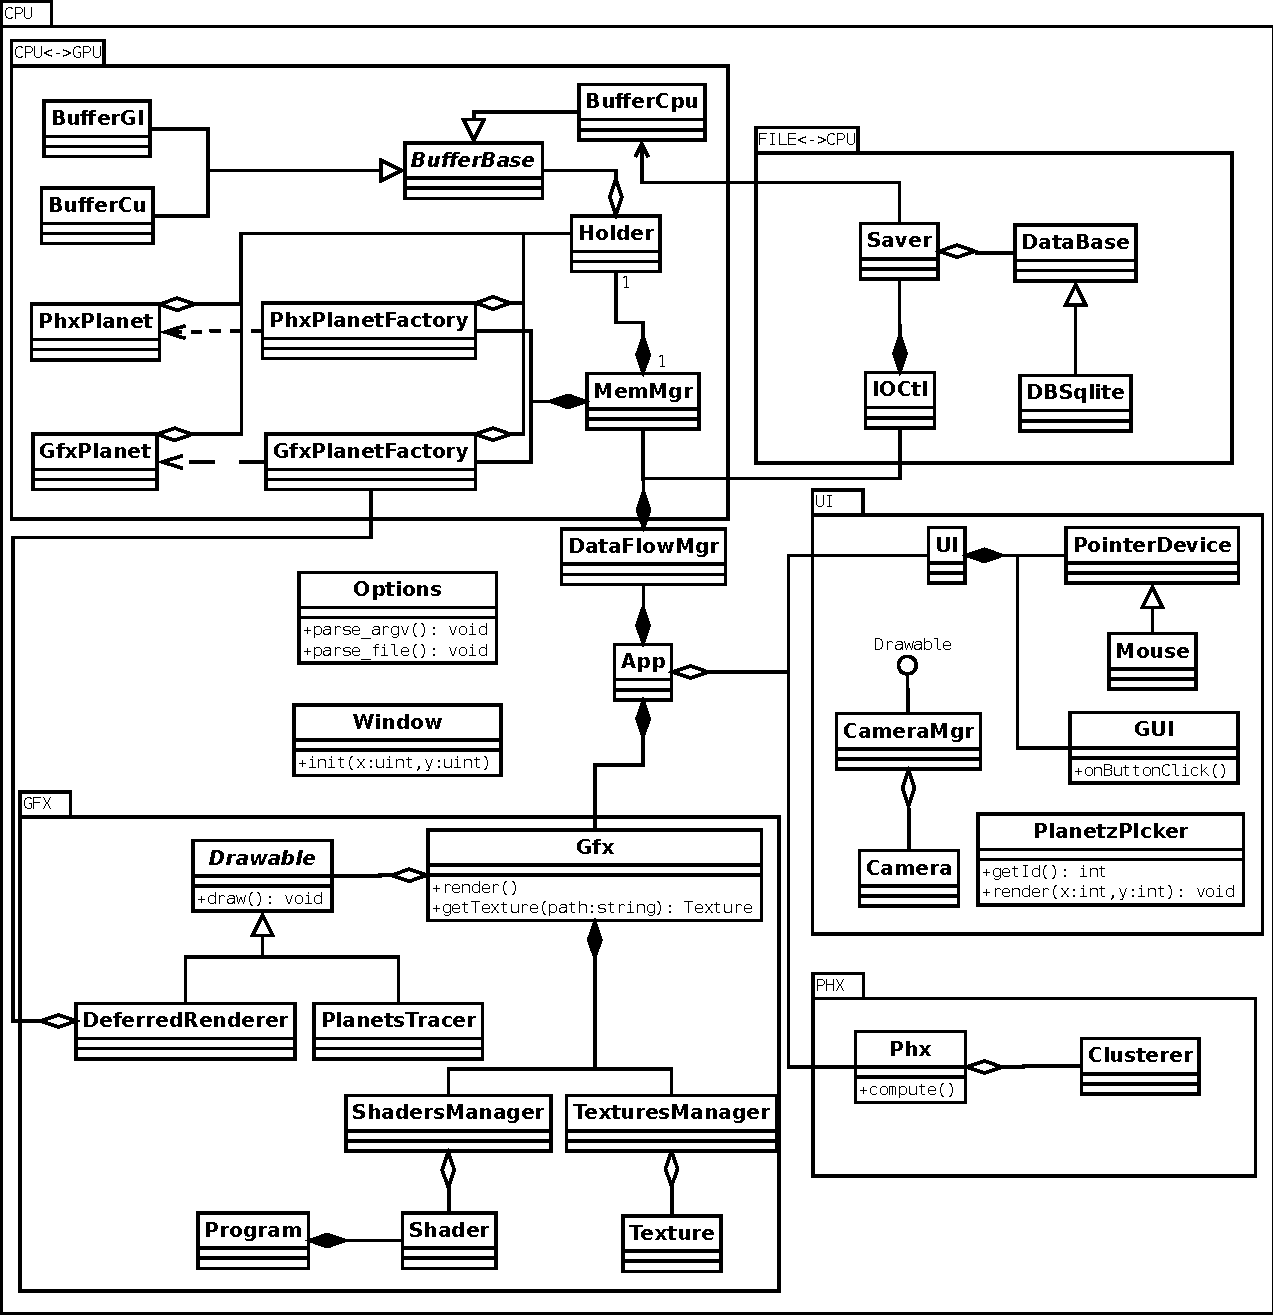
\includegraphics[width=\textwidth]{img/cpu_classes_revisited.pdf}
\caption{Aktualny diagram klas}
\label{fig:cpudiarev}
\end{figure}

\begin{description}
\item[\texttt{Window}] klasa powstała aby zarządzać oknem aplikacji.
\item[\texttt{Options}] tworzy obiekt konfiguracyjny na podstawie pliku i parametrów konsoli.
\item{}
\item[\texttt{GFX::DeferredRenderer}] jedyny moduł odpowiedzialny za rysowanie planet w każdej klatce. Zastąpił on poszczególne klasy, robiąc wszystko sam.
\item[\texttt{GFX::PlanetsTracer}] klasa służąca do zbierania i wyświetlania śladu za planetami. Powstała jako dodatkowa funkcjonalność z ciekawości jak zachowują się planety.
\item[\texttt{GFX::TexturesManager}] klasa przeniesiona z przestrzeni \texttt{FILE2CPU} z powodu wygody użytkowania. Agreguje już załadowane tekstury aby nie ładować tych samych kilka razy. Z uwagi na nowy silnik graficzny, jej użycie jest znikome.
\item[\texttt{GFX::ShaderManager}] analogiczna klasa do \texttt{TextureManager}a, tylko służąca do ładowania shaderów. Powstała po tym, jak niewygodne okazało się ich używanie.
\item[\texttt{GFX::Program}] reprezentuje program OpenGLa składający się z 2 lub 3 shaderów.
\item{}
\item[\texttt{UI::PlanetzPicker}] jest klasą odpowiedzialną za dowiadywanie się która planeta została wciśnięta myszką. Powstała po tym jak uznaliśmy że taka funkcjonalność jest bardzo przydatna.
\item[\texttt{UI::CameraMgr}] zastąpiła dawną klasę \texttt{GFX::Camera}. Dzięki niej możliwa jest zmiana kamer i zarządzanie nimi.
\item[\texttt{UI::Camera}] jest bazową klasą dla wszystkich rodzajów kamer.
\end{description}

